%% content.tex
%%

%% ===========================
\chapter{Konzeption}
\label{ch:Konzeption}
%% ===========================

Ein Konzept dient in der Softwarearchitektur zur Bildung eines abstrakten Systemmodells als Basis für die Umsetzung. Zur Gestaltung werden technische Details weggelassen und stattdessen allgemeingültige Begriffe und ihre Zusammenhänge definiert. Weiterhin wird ein Grundverständnis durch definieren von Strukturen und Konzepten gebildet. Zu Beginn der Überlegung werden Systemgrenzen festgelegt und beschrieben was Teil des System ist. Überdies werden Schnittstellen definiert, die Wechselwirkungen zwischen den Komponenten beschreiben. Weiterhin werden im Zuge der Überlegungen Technologien ausgewählt, die zur Umsetzung der verschiedenen Komponenten verwendet werden. Abschließend wird auf die Entwürfe der einzelnen Komponenten näher eingegangen.  

%% ===========================
\section{Architektur}
%% ===========================

Zuerst wird ein erster Überblick über den groben Aufbau des Systems gegeben. In Abbildung \ref{konzept_architektur} können die Zusammenhänge des abzubildenden Software-Systems betrachtet werden. Bei einer Betrachtung in der 3-Schichten-Architektur stellt der Browser und die Client.war die Darstellungsschicht dar. Die Fachkonzeptschicht ist in der Server.war umgesetzt. Die Datenbank befindet sich zwar auch in der Server.war, allerdings ist sie trotzdem unabhängig und kann jederzeit separat betrieben werden.

\begin{figure}[htbp]
\centering
  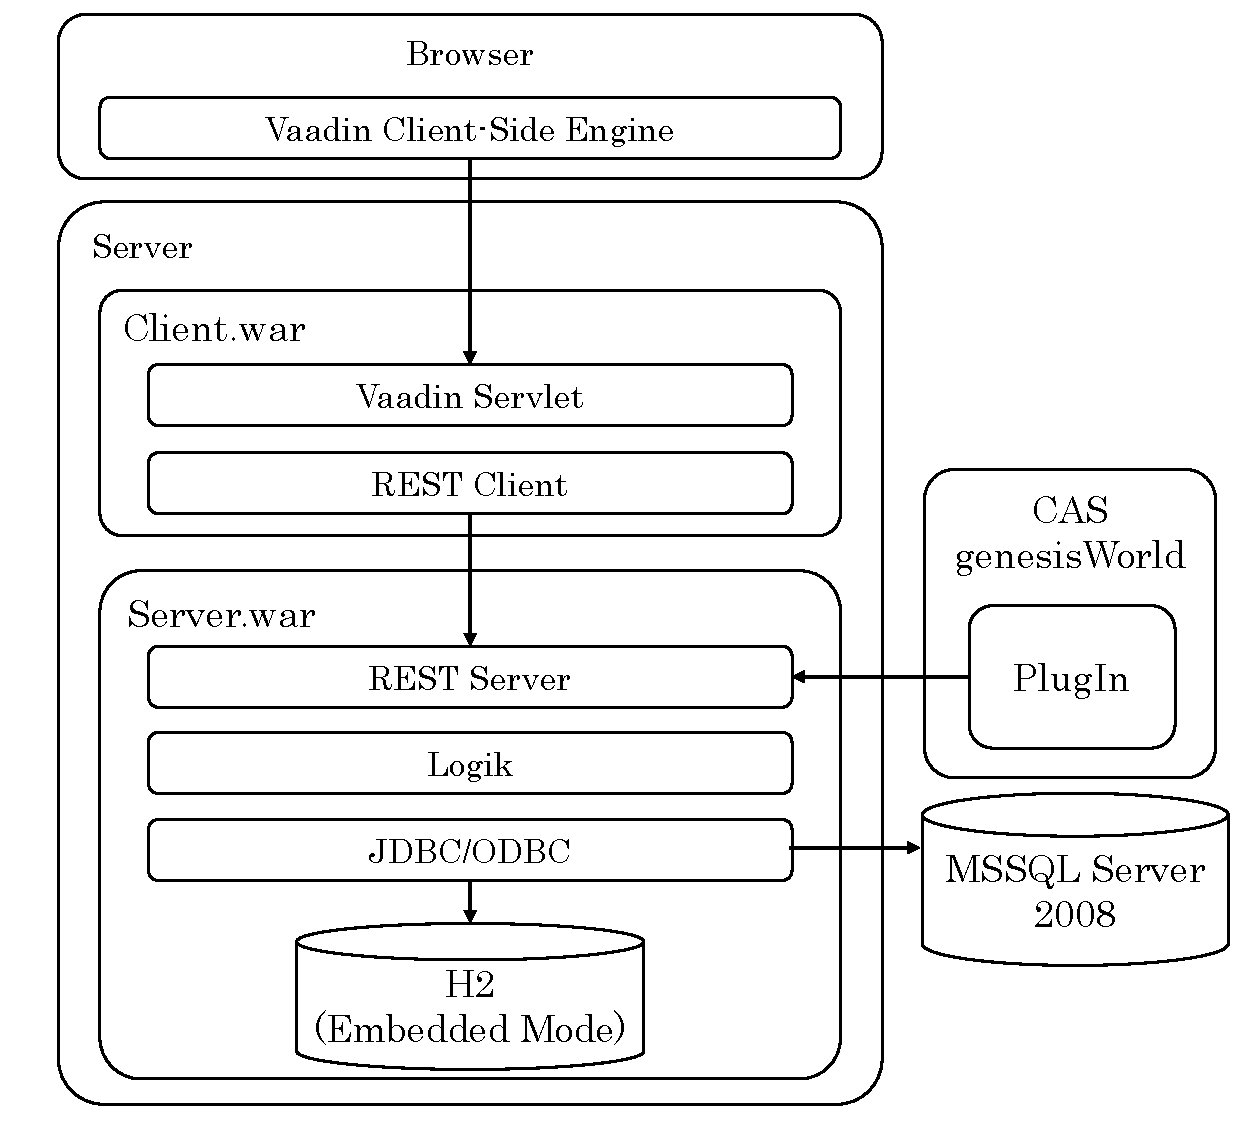
\includegraphics[width=0.8\textwidth, width=0.8\textwidth]{pics/Konzept_architektur.pdf}
\caption{Konzeptionelle Darstellung der Architektur}
\label{konzept_architektur}
\end{figure} 

Die Vaadin Client-Side-Engine verwaltet das Rendering der Oberfläche im Web-Browser, durch den Einsatz verschiedener clientseitiger Widgets, die das Gegenstücke zu den serverseitigen Komponenten bilden. Es leitet Benutzerinteraktionen an die Serverseite weiter und rendert anschließend die Änderungen für die Benutzeroberfläche. Die Kommunikation findet über asynchrone HTTP-oder HTTPS-Anfragen statt.

Serverseitig arbeitet die Vaadin-Anwendungen auf der Java-Servlet-API. Das Vaadin-Servlet oder genauer die Klasse \textit{VaadinServlet} ist für die Delegation verschiedenen Clients zuständig. Sie empfängt Anfragen und legt mithilfe von Cookies fest welche Benutzersitzung, zu welchem Client gehört.

Interaktionen mit dem Benutzer-Interface-Komponenten erzeugen Events, die zunächst auf der Clientseite durch Widgets verarbeitet werden. Nachfolgend werden die Events durch den HTTP-Server, das Vaadin-Servlet und durch die Komponenten der Benutzeroberfläche geleitet, bis sie zu den in der Anwendung definierten Event-Listenern gelangen. In den Listenern wird mithilfe des REST-Clients ein POST-Requests an die Logik gesendet. Dieser enthält alle in der Oberfläche definierten Parameter. 

In der Server.war werden REST-Requests entgegen genommen. Anhand der mitübertragenen Filteroptionen, werden die Bedingungen für die Datenbankabfrage zusammengestellt. Anschließend wird eine Verbindung zur H2-Datenbank aufgebaut. Das Ergebnis der Abfrage wird in das JSON-Format überführt und zurück an die Client.war geschickt. Dort angekommen werden die Daten an die Chart-Komponenten übergeben, was ein Neuaufbau der Komponente bewirkt.      

Eine der Anforderung ist die unabhängige Umsetzung von Client und Server. Der erste Schritt zur Umsetzung der geforderten losen Kopplung zwischen Darstellung und Logik, wird durch die Aufsplittung in zwei verschiedene Anwendungen erreicht. Die Client.war beinhaltet die Klassen und Objekte der Darstellung. Wohingegen die Server.war alle Elemente zur Umsetzung der Logik enthält. Die Verwendung des REST-Protokolls zwischen der Client.war und Server.war stellt den nächsten Schritt der losen Kopplung dar. Einer der Vorteile ist, dass Funktionen des Systems durch andere Clients genutzt werden können, ohne Änderungen am Server durchführen zu müssen. Beide WAR-Dateien werden in einem Apache-Tomcat-Webserver deployed und können über die dementsprechende URL angesprochen werden.

Die Logikkomponente in der Architektur stellt eine Zusammenfassung aller Funktionen des Anwendungskerns dar. Sie kümmert sich um die Generierung der Abfragen, welche an die Datenbank gestellt werden. Dabei erfolgt eine dynamische Generierung der Abfragen, um nicht durch unnötige Bedingungen die Abfragegeschwindigkeit zu verringern. Abfragen werden mithilfe der Java Database Connectivity(JDBC) an die Datenbank gestellt. Neben der Generierung der Abfragen enthält die Logikkomponente Funktionen zum Extrahieren und Transformieren der Daten, aus der alten Datenbank. Der ETL-Prozess wird nur einmalig ausgeführt, allerdings stellt er einen wichtigen  Schritte für die Umsetzung dar. 

Um nicht periodisch Extraktion und Transformation wiederholen zu müssen, wird ein selbstgeschriebenes Plugin im CAS genesisWorld Anwendungsserver eingesetzt. Die Grundidee des Plugins ist Benachrichtigungen über Änderungen an unser System zu übermitteln. Dort findet eine Kontrolle statt, die den Datensatz auf Relevanz prüft. Ist dies der Fall, besorgt sich die Anwendungslogik anhand der zuvor übermittelten GGUID alle benötigten Daten.

%% ===========================
\section{Technologien}
%% ===========================

Als einer der am meist verbreitetsten Programmiersprachen, stellt Java die Grundlage aller verwendeten Technologien dar. Zur Darstellung der Inhalte für den Client wird Vaadin verwendet. Der Apache Tomcat7 nimmt die Rolle des Anwendungsservers ein. Die Kommunikation auf Basis von RESTful Web Services wird mithilfe von Jersey realisiert. Weiterhin wird opencsv für das Lesen und Schreiben von CSV-Dateien verwendet. JDBC dient der Kommunikation zwischen Anwendungsserver und der Datenbank. Die H2-Datenbank stellt die Datenquelle des Systems dar. Im Folgenden werden alle Bestandteile bis auf den H2 der bereits erläutert wurde, näher beschrieben. 

\paragraph{Vaadin}

Vaadin ist ein Open-Source, Java basiertes Framework für den Aufbau von modernen Web-Anwendungen. Der Kerngedanke des Frameworks ist, dass die gesamte Anwendungslogik in der Serverseite einer Anwendung ausgeführt wird, während die Clientseite nur für das Senden der Benutzeraktionen an den Server und verantwortlich für die Reaktion auf die Antworten ist. Da es auf GWT basiert, kann sowohl der Client- und Server-Code in reinem Java geschrieben werden.

Die aktuelle Version von Vaadin, wurde im Februar 2013 veröffentlicht. Die folgenreichste Änderung von Vaadin6 war die Integration von GWT zu Vaadin, die eine bessere Unterstützung für die clientseitige Widget-Entwicklung bedeutet und sogar die Möglichkeit zu Erstellung von offline Vaadin-Anwendungen mit sich bringt.

Neben Open-Source, ist die im Unternehmen vorhandene Erfahrung ein Grund für die Wahl des Frameworks. Allerdings war VaadinCharts, eine Erweiterung für Vaadin, für die Auswahl ausschlaggebend. Es basiert auf Highcharts, einem JavaScript-Packet. Highcharts zeichnet sich durch eine umfangreiche Sammlung an Funktionen zur Darstellung von Diagrammen aus. 

\paragraph{Jersey}

Jersey RESTful Web Services ist ein Open-Source-Framework zur Entwicklung von RESTful Web Services in Java, die Unterstützung für JAX-RS-APIs bietet und die JAX-RS (JSR 311 und JSR 339)-Referenzimplementierung darstellt. JAX-RS-Annotationen werden verwendet um die REST Relevanz von Java-Klassen zu definieren. Jersey ist dabei die Referenzimplementierung dieser Spezifikation. Jersey enthält im Grunde einen REST-Server und einen REST-Client. Auf der Serverseite verwendet Jersey ein Servlet, das vordefinierten Klassen abtastet um REST-Ressourcen zu identifizieren. Über die web.xml Konfigurationsdatei werden die von der Jersey-Distribution bereitgestellten Servlets registriert. Diese Servlets analysieren die eingehenden HTTP-Anforderungen und wählen die richtige Klasse und Methode für die Anfragen aus. Diese Auswahl basiert auf Annotationen in den Klasse und Methoden. Weiterhin unterstützt JAX-RS die Erstellung von XML-und JSON, über die Java Architektur für XML Binding (JAXB).

\paragraph{Apache Tomcat7}

Tomcat ist ein Open-Source Webserver, entwickelt von der Apache Group. Der Apache Tomcat implementiert die Java-Servlet und die Javaserver-Pages(JSP) Spezifikationen von Sun Microsystems und ist daher ebenfalls eine Referenzimplementierung. Er stellt weiterhin eine rein auf Java basierende HTTP-Webserver Umgebung dar. Apache Tomcat enthält Tools für Konfiguration und Management, kann aber auch durch die Bearbeitung von XML-Dateien konfiguriert werden.

\paragraph{opencsv}

Da Java das Parsen von CSV-Dateien nativ nicht unterstützt, müssen wir auf Drittanbieter-Bibliothek zurückgreifen. Mit opencsv erhalten wir eine sehr einfache CSV-Parser-Bibliothek für Java. Die Bibliothek kann zum erstellen, lesen und schreiben von CSV-Dateien benutzt werden. Die beste Fähigkeit des opencsv-Parsers ist das Mapping von Ergebnissen auf Java-Bean-Objekte.

\paragraph{JDBC}

Die JDBC-API ermöglicht den programmgesteuerten Zugriff auf relationale Daten, direkt aus der Java Programmiersprache heraus. Durch Verwendung der JDBC-API können Anwendungen SQL-Anweisungen ausführen, Ergebnisse abrufen und die Veränderungen auf die Datenquelle zurückschreiben. Der JDBC-API kann auch mit mehreren Datenquellen in einer verteilten, heterogenen Umgebung interagieren. 

%% ===========================
\section{Datenbankdesign}
%% ===========================

Das Datenbankdesign stellt einen wichtigen Abschnitt der Konzeption dar. Festlegungen im Bereich des Datenmodells werden in dieser Phase getroffen. Sie entscheiden ob Anforderungen und Erwartungen erfüllt werden können. In dieser Phase sind die Charakteristika der Daten zu untersuchen und das Datenmodell entsprechend nach ihnen auszulegen.

%% ===========================
\subsection{Konzeptionelles Design}
%% ===========================

Normalisierung dient der Organisation von Feldern und Tabellen einer relationalen Datenbank, um Redundanz und Abhängigkeit zu minimieren. Die Kehrseite hingegen ist eine Steigerung des Aufwands, um die benötigten Daten wiederzugewinnen. Normalisierung bietet die Möglichkeit einen Austausch zwischen Performance und Stabilität des Datenbankmodells vorzunehmen. 
In unserem Fall stellt ersteres absolute Priorität dar. Daher wird versucht die Normalisierung so gering wie möglich zu halten. 

Die erste Überlegung hinsichtlich des Schemas ist, welche Daten für die Beantwortung der Abfragen benötigt werden. Der Datenbankdesigner steht bei analytischen System immer wieder vor der Entscheidung, wie viele Information aus dem alten System in das Neue übernommen werden sollten. Um höchst mögliche Performance zu erreichen werden lediglich die für das Szenario benötigten Daten extrahiert. Allerdings entsteht durch nachträgliches hinzunehmen von Funktionen ein erhöhter Aufwand für Änderungen am Schema und des ETL-Prozesses. Abbildung \ref{konzept_SchemaNeu} zeigt das für die Datenbank neu entworfene Schema. 

\begin{figure}[htbp]
\centering
  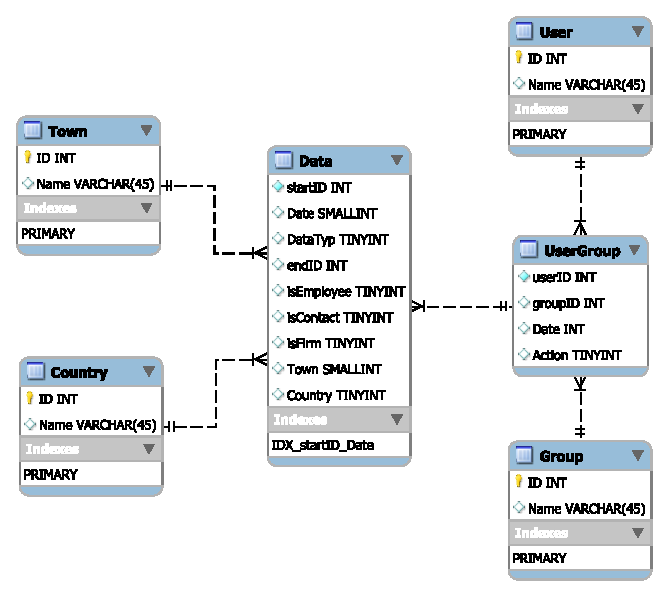
\includegraphics[width=0.8\textwidth, width=0.8\textwidth]{pics/NewSchema.pdf}
\caption{Neues Datenbankschema}
\label{konzept_SchemaNeu}
\end{figure} 

Die Idee hinter dem Schema ist die Verwendung einer einzelnen Tabelle zur Aufbewahrung der Informationen, der Verbindungsmerkmale. Diese Tabelle ermöglicht es ausgehend von einem Benutzer, alle Verbindungen zu anderen Personen zu finden. Im Grunde genommen sind vier Spalten dafür ausreichend. Die erste Spalte \textit{startID} beinhaltet die Person, von der die Suche ausgeht. Eine Zuordnung der Tupel zu einem Datum erfolgt über die Spalte \textit{Date}. Um Verbindungsmerkmale zu unterscheiden werden Zahlen von 1 bis 5, für die jeweiligen Verbindungsmerkmale, in der Spalte \textit{DataTyp} verwendet. Die letzte Spalte \textit{endID}, beinhaltet die Personen zu denen die Verbindungsmerkmale letztendlich führen. Anderen Spalten wie z.B. \textit{Town} oder \textit{Country} dienen lediglich der Filterung der Ergebnisse.

Um mit den geringeren Speicherkapazitäten die uns zur Verfügung stehen zurechtzukommen, wird auf das Problem der Datenredundanz eingegangen. Durch Normalisierung lässt sich Datenredundanz zwar nicht verringern, allerdings kann man sie in kontrollierbare Bahnen lenken. Im neuen Schema wurden solche Maßnahmen auf die Spalte \textit{Town} und \textit{Country} angewendet. Beide Spalten werden voraussichtlich Millionen von Werten beinhalten. Allerdings gibt es nur 193 Länder auf der Welt. Wörter wie Deutschland werden sich daher sehr oft wiederholen. Die Spalte \textit{Country} ist vom Datentyp \texttt{Varchar}, welches pro Zeichen 2 Byte benötigt. Das wären beim Wort Deutschland 22 Byte. Legt man nun für die Spalte \textit{Country} eine neue Tabelle an, wird in dieser jedes Land nur einmal vermerkt. Jedes Land bekommt einen Schlüssel in Form einer Zahl. In der eigentlichen Tabelle Data werden nur noch die Zahlen, anstatt den vollständig ausgeschrieben Wörtern verwendet. Das würde beispielsweise bei dem Wort "Deutschland" eine Reduktion von 22 Byte auf 1 Byte bewirken. Die Reduzierung auf 1 Byte lässt sich auf das \texttt{tinyint}-Format zurückführen. Das gleiche gilt für die Spalte \textit{Town}. Bei ihr wird allerdings der Datentyp \texttt{smallint} verwendet, mithilfe dessen ein Zahlenbereich von -32768 bis 32767 abgebildet werden kann. Die Spalten \textit{isEmployee}, \textit{isContact} und \textit{isFirm} können nur zwei verschiedene Zustände darstellen. Trifft zu oder trifft nicht zu. Der Datentyp \texttt{bool} reicht daher zur Abbildung der zweiwertigen Zustände aus. Ein Feld vom Datentyp \texttt{datetime} benötigt 8 byte an Speicher. Um hier ebenfalls Einsparungen vorzunehmen, wurde beschlossen das Datum als \texttt{smallint} zu deklarieren. Dies ist möglich da nur der Tag innerhalb des Datums von Interesse ist. Dazu wird ein frei gewählter Nullpunkt festgelegt. In unserem Fall wurde der 01.01.1990 als Nullpunkt gewählt, da keine älteren Daten existieren, die Relevanz besitzen. Darauf aufbauend wird das Datum, durch die Differenz in Tagen zum Nullpunkt, in der Spalte \textit{Date} abgelegt. Die Hochrechnung der Tabelle \ref{tb_speicherplatzverbrauch} zeigt, dass durch die Normalisierung der Speicherplatzverbrauch um bis zu $ \frac{1}{6} $ gesenkt werden kann.


Möchte man nun die Abfrage eines Benutzers die eine Filterung anhand einer Stadt voraussieht beantworten, muss man zuerst an die \textit{ID} der Stadt herankommen. Dabei können zwei verschiedene Ansätze verfolgt werden. Der erste Ansatz wäre ein Join zwischen \textit{Town} und \textit{Data}, um direkt mit dem Namen der Stadt zu arbeiten. Diese Variante dürfte aufgrund des Kreuzproduktes von Millionen von Zeilen nicht sehr performant sein. Eine andere Möglichkeit ist, eine separate Abfrage an die Datenbank zu stellen, in der die \textit{ID} zum Namen ermittelt wird. Mithilfe der \textit{ID} kann dann ohne einen Join die Ergebnismenge ermittelt werden. Dieser Ansatz dürfte vor allem durch die Abwesenheit von Netzwerkzugriffen zu höheren Abfragegeschwindigkeiten führen. Dieses Vorgehen kann für die Stadt, das Land und die Gruppenzugehörigkeit angewendet werden.

\begin{table}[htbp]
\centering
\begin{tabulary} {\linewidth} {l  r  C  l  C  r}
& & & & & \\
\multicolumn{6}{l}{Speicherplatzverbrauch ohne Normalisierung}\\
& & & & & \\
Zeitpunkt(timestamp) & 8 byte & x & 18.000.000 & = & \textasciitilde 137 MB \\  
Stadt(varchar) & 16 byte & x & 18.000.000 & = & \textasciitilde 343 MB \\  
Land(varchar) & 20 byte & x & 18.000.000 & = & \textasciitilde 274 MB \\  
\midrule
& & & & Summe & \textasciitilde 754 MB\\
& & & & & \\
\multicolumn{6}{l}{Speicherplatzverbrauch mit Normalisierung}\\
& & & & & \\
Zeitpunkt(smallint) & 2 byte & x & 18.000.000 & = & \textasciitilde 34 MB \\  
Stadt(integer) & 4 byte & x & 18.000.000 & = & \textasciitilde 72 MB \\  
Stadt(varchar) & 16 byte & x & 21.000 & = & \textasciitilde 0,32 MB \\  
Land(tinyint) & 1 byte & x & 18.000.000 & = & \textasciitilde 17 MB \\  
Land(varchar) & 20 byte & x & 218 & = & \textasciitilde 0,004 MB \\
\midrule  
& & & & Summe & \textasciitilde 123 MB\\
& & & & & \\
\end{tabulary}
\caption{Vergleich des Speicherplatzverbrauchs}
\label{tb_speicherplatzverbrauch}
\end{table}

Die Tabelle \textit{GroupDate} unterscheidet sich von den anderen Tabellen wie \textit{Town} oder \textit{Country}, da in dieser noch weitere Details vermerkt sind. Diese ermöglichen es die Zusammenstellung von Gruppen über die Zeit nachzuvollziehen. In der Spalte \textit{Action} wird festgelegt ob die Tupel einen Eintritt oder einen Austritt einer Person darstellt. Die Spalte \textit{Date} beinhaltet das Datum des Ereignisses. Mithilfe beider Attribute lassen sich Gruppenzusammensetzung auf bestimmte Zeitpunkte bezogen rekonstruieren.

%% ===========================
\subsection{Zugriffsstrukturen}
%% ===========================

Indizes dienen der Beschleunigung von Suchen nach bestimmten Spaltenwerten. Ohne Indizes müsste die H2-Datenbank beim ersten Datensatz beginnen und dann die gesamte Tabelle durchgehen, um eine Abfrage zu beantworten. Je größer die Tabelle ist, desto höher sind die Kosten dafür. Daher bietet der Einsatz sich gerade in Anbetracht nach der Forderung von hoher Abfragegeschwindigkeit an. Jeder Index bedeutet allerdings einen Zuwachs im Speicherplatzverbrauch. Zur Indexierung der Tabellen \textit{Town}, \textit{Country}, \textit{User} und \textit{Group} eignen sich Hash-Indizes. Sie bieten einen extrem schnellen Zugriff auf die Daten. Diese Schnelligkeit ergibt sich aus der Verwendung von Berechnungsvorschriften, zur Ermittlung der Position des gesuchten Wertes. Indizierungen sollen in unserem Schema über die Spalten mit der Bezeichnung \textit{Name} in den jeweiligen Tabellen vorgenommen werden, da der Client mit dem Namen anstatt der ID arbeitet. Mithilfe des Namen wird deshalb die zugehörige ID ermittelt. Die Nutzung von Hash-Indizes bringt allerdings Limitierungen mit sich. Eine der wichtigsten ist, dass sie nur für Vergleiche("=") verwendet werden können. Somit werden keine Wertebereich-Abfragen("<" oder ">") unterstützt. Es gibt allerdings noch andere Nachteile \cite{SWB-352401869}, auf die aber in dieser Arbeit nicht näher eingegangen wird. 

Für die Tabelle \textit{UserGroup} eignet sich der B\textsuperscript{+}-Baum Standard-Index von H2. Dieser kann für die Spalte \textit{userID} verwendet werden, der den ersten Wert einer Suche darstellt. Der B\textsuperscript{+}-Baum-Index eignet sich auch für die Tabelle \textit{Data}. Hier ist außerdem die Verwendung eines Mehr-Attribut-Indexes vorgesehen. Der Vorteil eines Mehr-Attribut-Indexes ist, dass bei einer Punkt-Abfrage über alle Zugriffsattributwerte nur ein Indexzugriff erfolgen muss. Indexiert werden in unserem Fall die Spalte \textit{startID} und \textit{Date}. Beide Spalten sind sortiert und bieten sich somit für die Verwendung eines geclusterten Index an. Geclusterte Indizes sind in der gleichen Form sortiert wie die interne Relation. Ein geclusterter Index unterstützt Bereichsanfragen sehr gut, was bei der Beschränkung auf Zeitspannen von Vorteil sein dürfte.       


%% ===========================
\section{Extract Transform Load Prozess}
%% ===========================

Daten der operativen Systeme unterstützen die wertschöpfenden Geschäftsprozesse innerhalb eines Unternehmens. Sie sind demnach auf die Steuerung und Überwachung des Tagesgeschäftes ausgerichtet und daher transaktionsbezogen. Somit sind die Daten in ihren Begrifflichkeiten häufig nicht vergleichbar und ihrer Bewertung sowie Konsolidierung unterschiedlich. Um die Daten dennoch für analytische Zwecke einzusetzen, ist eine Überführung in eine geeigneter Struktur von Vorteil. Eine solche Überführung wird in der Literatur als Extract-Transform-Load(ETL)-Prozess bezeichnet \cite{ElSappagh201191}. 

%% ===========================
\subsection{Extract}
%% ===========================

Zunächst dient die Extraktion primär der Beschaffung von Daten, aus dem MSSQL Server. Überdies können durch den Prozess Daten bereits reduziert,  zusammengeführt und ersetzt werden. Für eine zutreffende Formulierung der Abfragen, müssen Besonderheiten in die Ermittlung der Daten beachtet werden. Eine vollständige und korrekte Datenmenge stellt die Grundlage jeder guten Analyse dar.

Die erste Besonderheit stellt die Analyse über Zeiträume hinweg dar. Es gilt dabei die Veränderungen der Daten über die Zeit zu berücksichtigen. Die Tabelle  \textit{Changelogbook} ermöglicht es Veränderungen in den Datensätzen nachzuvollziehen. Eine solche nachvollziehbare Veränderung ist in der Gruppenzusammensetzung zu finden, aufgrund von Abgängen und Zugängen von Personen. Neben den Datensätze die über die Zeit verändert wurden, existieren Datensätze die sich über längere Zeiträume erstrecken. Termine wie Tagungen beispielsweise, erstrecken sich über mehrere Tage. In der MSSQL-Datenbank werden diese Termine in einer Tupel aufbewahrt. Bei unserer Analyse hingegen stellt jede Tupel eine Verbindung zu einem bestimmten Zeitpunkt in Tagen dar. Somit muss ein Datensatz der sich über mehrere Tage erstreckt, in der H2-Datenbank durch mehrere Tupeln repräsentiert werden. Aufgrund dessen muss im Ergebnis der SQL-Abfrage die Anzahl der Tage vermerkt werden. In späteren Transformationen kann mithilfe dieser Angaben die entsprechende Anzahl an Tupeln erzeugt werden.

Eine weitere Besonderheit ergibt sich durch ein nicht im System vorgesehenes Verhalten der Benutzer, welche die Auswertung der Daten erschwert. CAS genesisWorld ermöglicht es Termine zu schieben. Diese Funktion wird von manchen Nutzern missbraucht. Anstatt für einen ähnlichen Termin einen neuen Eintrag anzulegen, wird ein alter Termin aus Bequemlichkeit geschoben. Das hat zur Folge, dass Termine die tatsächlich statt gefunden haben, in der Datenbank nicht mehr existieren. Um trotzdem diese Termine zu berücksichtigen wurde folgendes Konzept erarbeitet. Dem \textit{Changelogbook} lässt sich entnehmen ob die Felder \textit{start\_dt} und \textit{end\_dt} verändert wurden. Zur Feststellung ob ein Termin stattgefunden hat und anschließend geschoben wurde, müssen zwei Bedienungen erfüllt sein. 
Die erste ist der Zeitpunkt der Schiebung, die nach dem Termin liegen muss. Wird ein Termin aus anderen Gründen geschoben, findet dies in der Regel vor dem Start des Termines statt, damit die Personen nicht unnötig zum Termin erscheint. Die zweite Bedingung ist, dass der neue Termin in der Zukunft liegen muss. Neben den beiden Bedingungen ist zu beachten, ob die Operation auf den Datensätzen ein Update war. Nur dann ist der Datensatz von Relevanz für die Abfrage. 

Die Ergebnisse sämtlicher Extraktionen sollen in CSV-Dateien abgespeichert werden. Damit werden unter anderem Fehlersuchen vereinfacht. Weiterhin wird die Belastung des Hauptspeichers verringert, da nicht alle Ergebnisse bis zum Schluss des ETL-Prozesses in der Java-Laufzeitumgebung aufbewahrt werden müssen.

%% ===========================
\subsection{Transform}
%% ===========================

Zu Beginn der Transformation werden Filterungen durchgeführt. Unter der Filterung von operativen Daten versteht man eine Bereinigung syntaktischer oder inhaltlicher Defekte, der zu übernehmenden Daten. Die MSSQL-Datenbank besteht zu 37\% aus Nullwerten und zu 4\% aus leeren Feldern. Daten die beispielsweise Nullwerte enthalten und für die Ermittlung des Datums benötigt werden, sind für die Analyse nicht zu gebrauchen. Sie können daher im laufe des Prozesses aus den Daten entfernt werden. Bei den anderen Filteroperationen können Nullwerte vernachlässigt werden, da sie zweckmäßig abdingbar sind.

Der nächste Schritt wäre die Harmonisierung der Daten. Unter anderem besitzen die Telefonnummern kein einheitliches Format. Sie wurde manuell von Sachbearbeitern eingetragen. Das erfordert ein zusammenführen aller Nummern in ein einheitliches Format, welches einen automatischen Vergleich ermöglicht. Die Verbindungsmerkmale müssen ebenfalls in eine einheitliche Form gebracht werden. Spalten die gleiche Inhalte besitzen, aber unterschiedlich bezeichnet sind, müssen unter einer Bezeichnung zusammengeführt werden. 

Die in der Extraktion genannten Besonderheiten werden durch unterschiedliche Datenbankabfragen ermittelt. Dies führt zu vielen separaten Dateien. Zur Nutzung der Daten sind sie zum Abschluss der Transformation zusammenzuführen. Das Ergebnis wird anschließend in einer CSV-Datei gespeichert, welche die Basis für das Befüllen der H2-Datenbank bildet. 

%% ===========================
\subsection{Load}
%% ===========================

Beim Laden der Datensätze in die H2-Datenbank kommt ein sogenannter "bulk load" zum Einsatz. Dieser wird häufig zum laden von großen Datenmengen aus einer Datei in eine Datenbank eingesetzt. Er ermöglicht ein wesentlich schnelleres befüllen der Datenbank bei großen Datenmengen, als wie üblicherweise mit INSERT-Operatoren.

%% ===========================
\section{Synchronisation des Datenbestandes}
\label{ch:Konzeption:sec:updatedatenbestand}
%% ===========================

Systeme die auf dem Datenbestand anderer Systeme aufbauen, können zwei verschiedenen Ansätze zur Sicherstellung ihrer Aktualität verfolgen. Unser nebenläufiges System bezeichnen wir als A und den CAS genesisWorld Anwendungsserver als B. Einer der Ansätze ist die Intervall basierte Nachfrage über Veränderungen von A. Hierbei fragt A bei B zu festgelegten Zeitpunkten nach, ob Daten verändert wurden. Die Definition eines optimalen Intervalls stellt eine der größten Schwierigkeiten dar. Ist der Intervall zu groß, sinkt die Aktualität des Datenbestandes. Ist er zu klein, entsteht  ein starke Belastung für B. Der andere Ansatz ist A über Veränderungen an den Datensätzen von B zu informieren. Dadurch werden keine unnötigen Abläufe angestoßen, da nur im Falle einer Manipulation eines Datensatzes Prozesse in Bewegung gesetzt werden. Zwar wird die Aktualität der Daten gewährleistet, jedoch büßt A an Entscheidungsfreiheit ein. A kann nicht mehr selbst entscheiden wann aktualisiert wird. Der zweite Ansatz ist zwar effizienter, jedoch nicht immer umsetzbar. Das kann technische oder unternehmenspolitische Gründe haben, die notwendige Veränderung am Legacy-Systems ausschließen.  

\begin{figure}[htbp]
\centering
  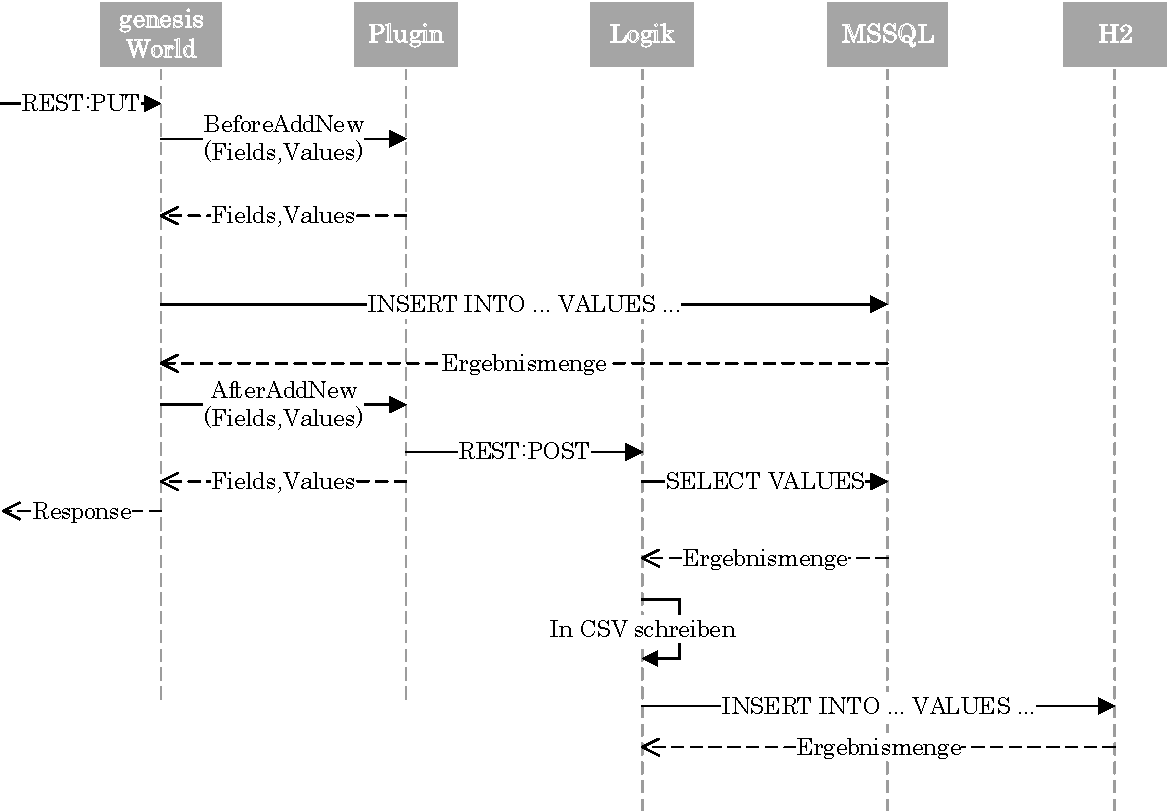
\includegraphics[width=1.0\textwidth, width=1.0\textwidth]{pics/sequenzdiagramm.pdf}
\caption{Sequenzdiagramm für einen neuen Datensatz}
\label{konzept_sequenz}
\end{figure}

In CAS genesisWorld gibt es eine Möglichkeit den zweiten Ansatz umzusetzen. Die Idee dabei ist den Applikationsserver um ein sogenanntes Plugin zu erweitern, welches über Veränderungen in den Datensätzen benachrichtigt wird. Ein solches Plugin kann als COM-Objekt mithilfe des Interfaces \textit{IGWSDKDataPlugIn} realisiert werden. Das resultierende COM-Objekt wird im Server von CAS genesisWorld registriert. Der Server delegiert, wie in Abbildung \ref{konzept_sequenz} zu sehen, bei einer Datenoperation den Aufruf an die für die jeweiligen Tabellen registrierten Plugins. Das Plugin selbst soll einen REST-Client besitzt, der einen POST an die Logik sendet. Er enthält die \textit{GGUID} des Veränderten Datensatzes. Mithilfe dessen die Extraktion des betroffenen Datensatzes angestoßen werden soll. Geplant ist neue Datensätze zuerst in einer CSV-Datei zwischenzuspeichern und anschließend in die H2-Datenbank einzufügen. Aktualisierungen der H2-Datenbank können auf der momentanen Datenbasis nur durch Erfassung neuer Datensätze aus dem MSSQL Server umgesetzt werden. Um auch Updates zu berücksichtigen müsste zu jeder Tupel die entsprechende \textit{GGUID} vorhanden sein. Ohne die \textit{GGUID} ist eine Zuordnung der Datensätze zwischen den Datenbanken nicht möglich. In diesem Fall wurde entschieden, dass dies kein Problem darstellt und es ausreichend ist die neuen Datensätze zu erfassen.

%% ===========================
\section{Darstellungskonzepte}
\label{ch:Konzeption:sec:Darstellungskonzepte}
%% ===========================

Bei der Konzeption einer Darstellung ist die Grad der Granularität von Informationen ein wichtiger Leitfaktor, zur Bestimmung des Aufbaus. In unserem Fall ist nicht die Eigenschaft eines Verbindungsmerkmals von interessiere, sondern ihr Typ und ihre Häufigkeit zu einer bestimmten Person. Da keine Detailinformationen zum Verbindungsmerkmal vorhanden sind, kann jeder Benutzer frei wählen von welcher Person ausgehend die Analyse stattfinden soll. Für die Oberfläche bedeutet dies einen Einstiegspunkt in Form eines Fensters, in dem der jeweilige Benutzername von dem die Suche ausgehen soll, eingegeben wird. Zusätzlich soll die IP-Adresse und Portnummer des Server angebbar sein, falls sich dieser auf einem anderen Rechner befindet.

Nach der Anmeldung findet eine Weiterleitung auf die eigentliche Seite statt. Dessen Aufbau ist in Abbildung \ref{konzept_darstellung} (a) zu sehen. Im oberen Bereich auf der Seite sind alle Regler, CheckBoxen und Eingabefelder zur Filterung der Ergebnismenge zu finden. Direkt darunter befindet sich ein Diagramm, welches die Ergebnismenge einer Abfrage visualisieren soll.

\begin{figure}[htbp]
\subfigure[Grober Entwurf des Aufbaus der Hauptseite]{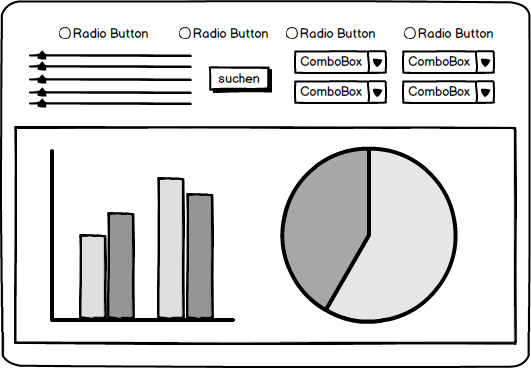
\includegraphics[width=0.49\textwidth]{pics/konzept_mockup.png}}\hfill
\subfigure[Tortendiagramm]{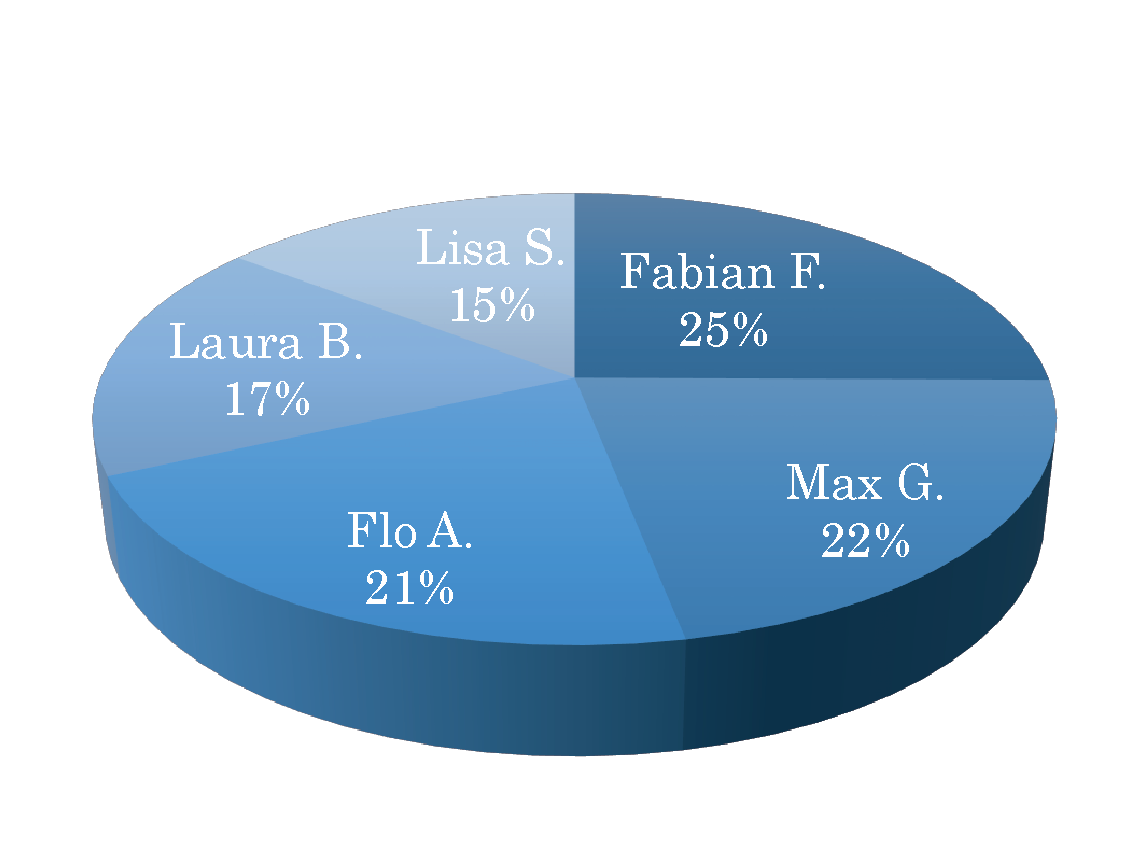
\includegraphics[width=0.49\textwidth]{pics/konzept_tortendiagramm.pdf}}\hfill
\subfigure[Balkendiagramm]{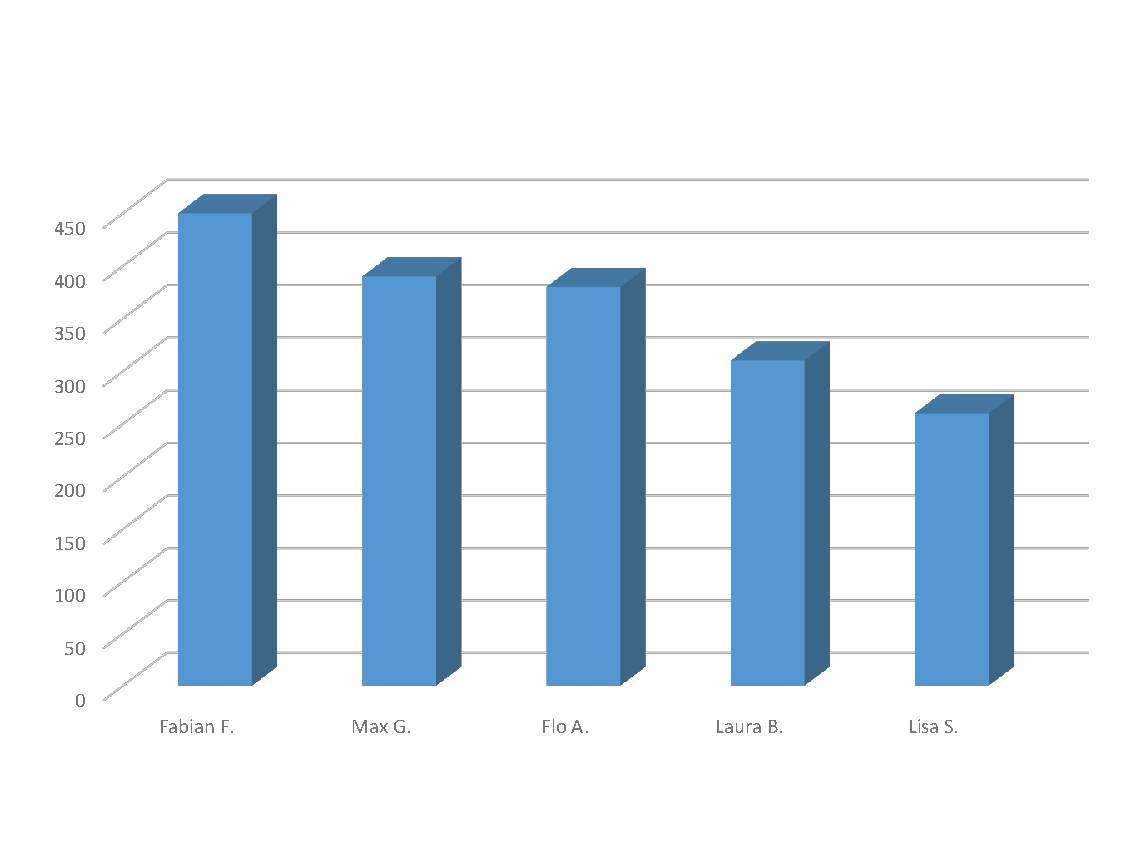
\includegraphics[width=0.49\textwidth]{pics/konzept_balkendiagramm.pdf}}\hfill
\subfigure[Tree Map]{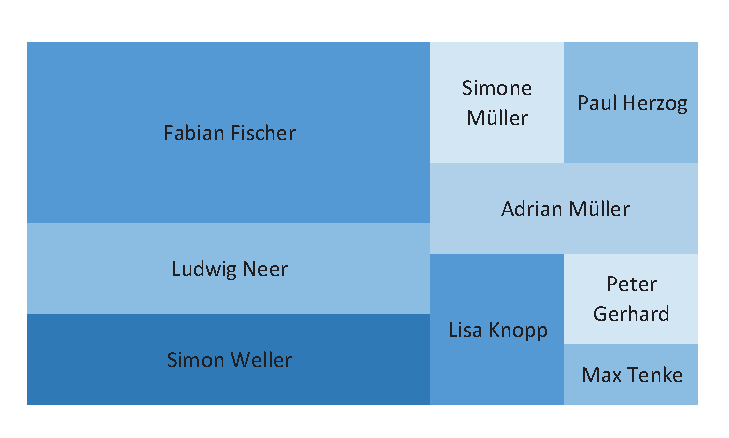
\includegraphics[width=0.49\textwidth]{pics/konzept_tree_map.pdf}}\hfill
\subfigure[Liniendiagramm]{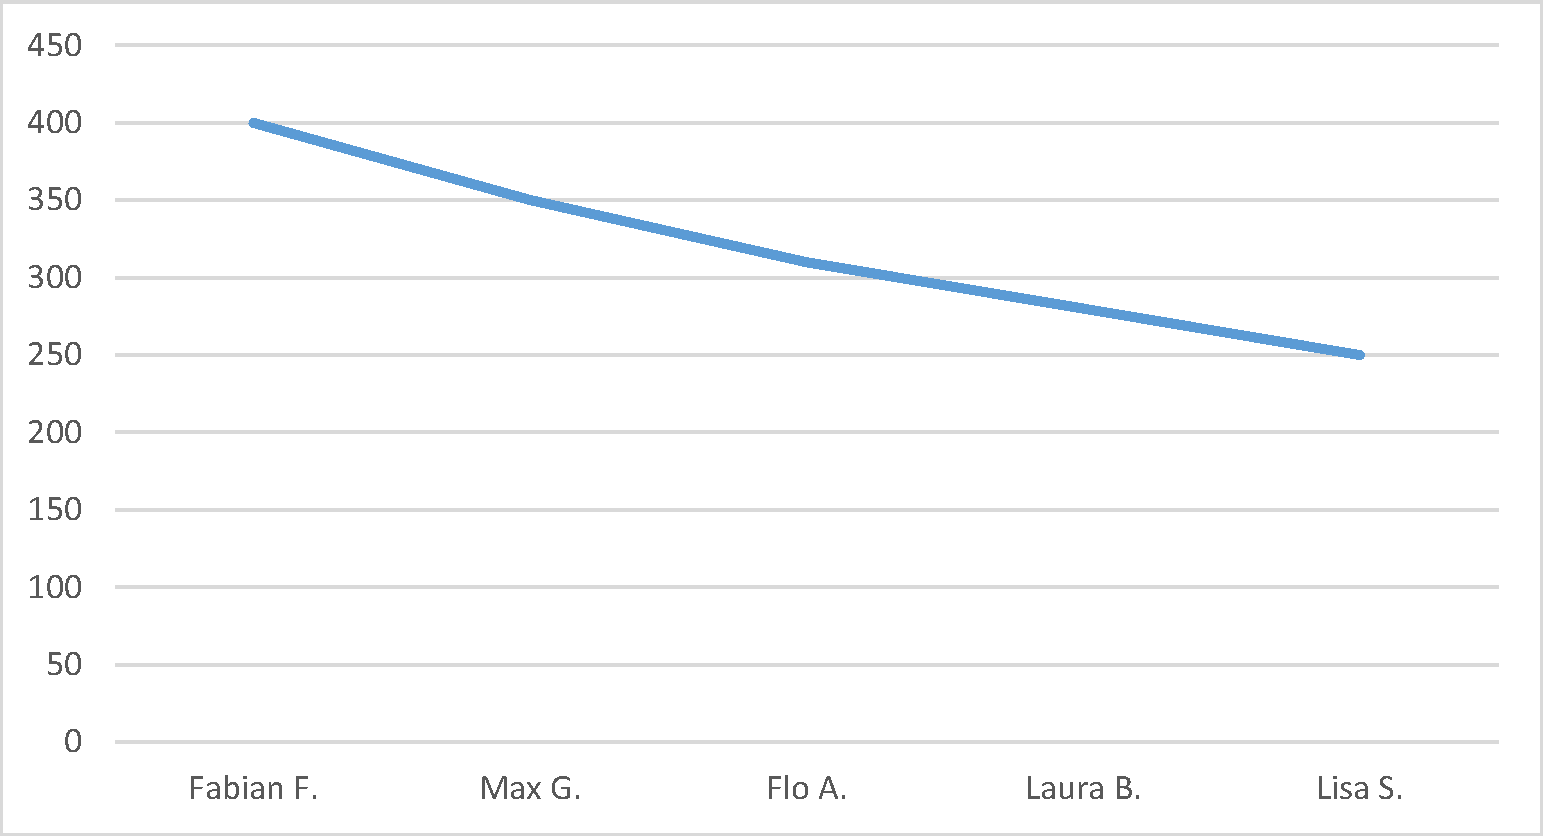
\includegraphics[width=0.49\textwidth]{pics/konzept_liniendiagramm.pdf}}\hfill
\subfigure[Netzdiagramm]{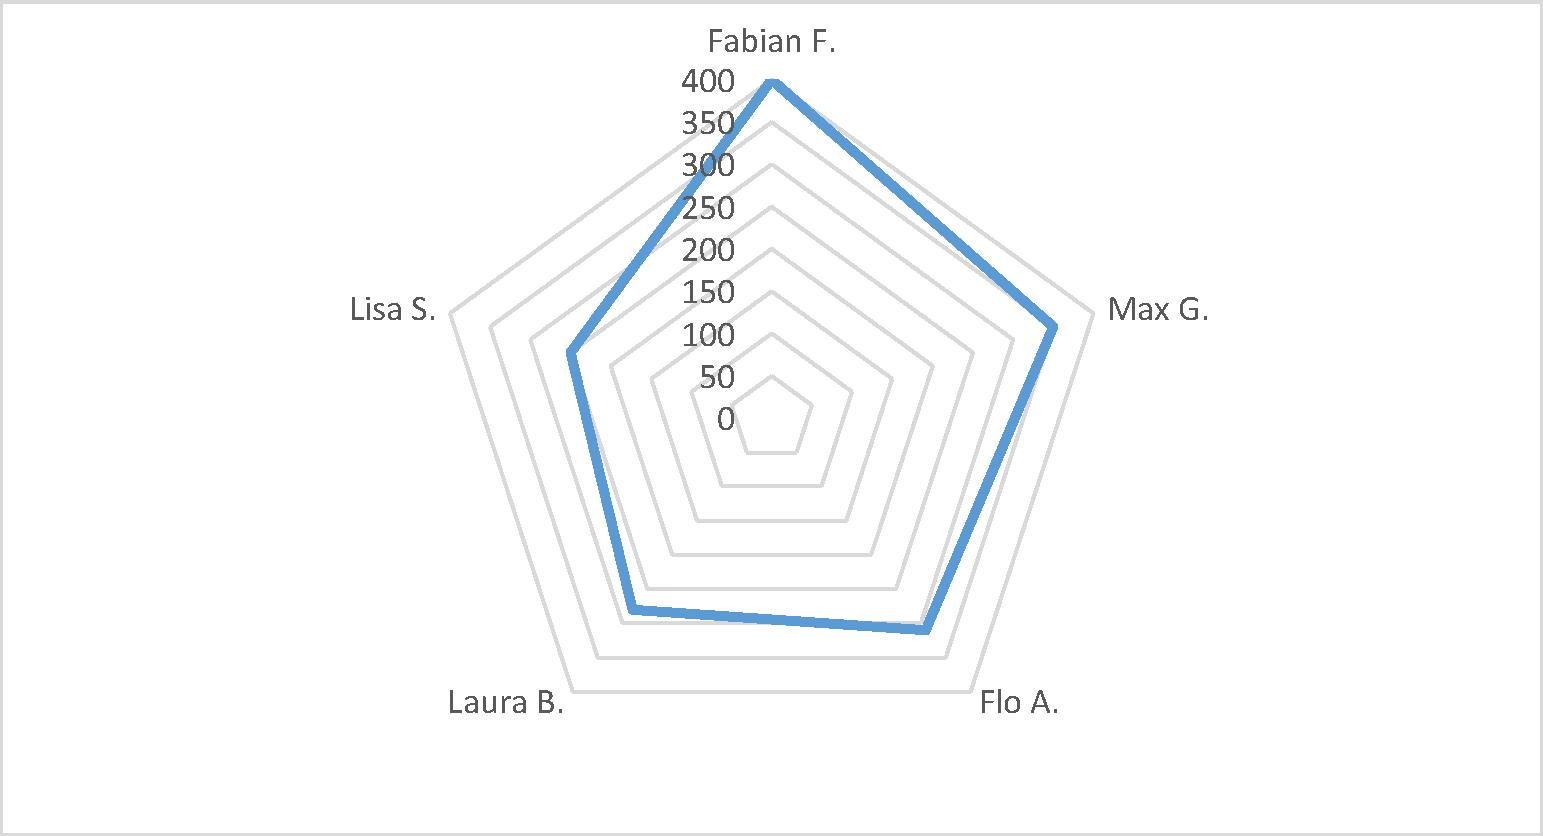
\includegraphics[width=0.49\textwidth]{pics/konzept_netzdiagramm.pdf}}
\caption{Entwürfe für die Oberfläche}
\label{konzept_darstellung}
\end{figure}

Diagrammtypen gibt es viele allerdings ergeben sich Einschränkungen durch die Verwendung eines Framework. Im Prinzip lässt sich jede Darstellung verwirklichen, allerdings ist das Aufwand-Nutzen-Verhältnis zu berücksichtigen. In einer Vorauswahl wurden einige umsetzbare Typen ausgewählt die in Abbildung \ref{konzept_darstellung} (b)-(f) dargestellt sind. 

Netzdiagramme geben Eigenschaften verschiedener Systeme wieder. Sie eignen sich daher gut zur Darstellung von Ausprägungen. Für unsere Form der Daten ist diese Darstellung gänzlich ungeeignet, da mit Mengen gearbeitet wird. 

Mithilfe von Liniendiagrammen lassen sich Trends und Zeitreihen darstellen. Die Verwendung verschiedener Linien ermöglicht zudem, die Darstellung mehrerer Trends. Die Benutzung dieses Diagramms macht keinen Sinn, da die Ergebnismenge sich nicht auf verschiedene Zeitpunkte bezieht, sondern die Summe der Werte aus einer Zeitreihe beinhalteten soll. 

Bei einer Tree Map steht jede Fläche eines Rechtecks im proportionalen Zusammenhang zur Gesamtfläche. Die Beachtung von Größenverhältnissen stellt einen nützliche Eigenschaft für unsere Daten dar. In unserem Fall würde jedes Rechteck aus dem jeweiligen Anteilen der Verbindungsmerkmale bestehen oder mithilfe eines Drilldowns
\footnote{Als Drilldown wird im Allgemeinen die Navigation in hierarchischen Daten bezeichnet. Auf Oberflächen bezogen wird damit die Darstellung von Detailinformationen durch einem Klick auf Darstellungselemente ausgedrückt. }
 die Verbindungsmerkmale aufzeigen. Beispielweise könnte die Person Ludwig Neer wiederum in Rechtecke unterteilt werden, mit der jeweiligen Anzahl der verschiedenen Verbindungsmerkmale. Das würde allerdings schnell zu einer schlechten Übersicht führen, da zu viele Kacheln zu einer schlechten Übersicht führen. Wird in einer Tree Map die Drilldown-Navigation gewählt, ist die Übersicht aller Informationen auf einen Blick nicht mehr gegeben. Aufgrund der Nachteile in der jeweiligen Variation wurde sich gegen den Einsatz einer Tree Map entschieden.

Kreisdiagramme ermöglichen eine Betrachtung der Gesamtheit zu ihren Einzelstücken, da der Kreis ein geschlossenes System darstellt. Allerdings müssen alle Teile sich auf die gleiche Basis beziehen. Es eignet sich hervorragend zur Darstellung von Verhältnissen. Wird nun eine weitere Unterteilung der Teilwerte gefordert, geht die Übersicht verloren. Um das zu vermeiden wird die unterteilte Teilmenge häufig in separaten Ansichten dargestellt. Allerdings steigt dadurch der Aufwand für den Nutzer in der Bedienung des Systems. 

Am besten dürfte sich ein Balkendiagramm eignen. Reihenfolgen beispielsweise lasse sich durch die resultierenden Stufen sehr gut darstellen. Balken selbst lassen sich außerdem in einzelne Teile aufspalten, ohne die Übersichtlichkeit zu verringern. Gegenüber dem Kreisdiagramm kann es zwar keine Betrachtung des Gesamten liefern ,allerdings ist das in diesem Anwendungsfall auch nicht nötig. 